\section{Trading Environment}
We build a trading environment compatible with Open AI Gym \cite{brockman2016openai} that serves two primary goals. The first objective is to translate domain-specific inputs into state/reward as inputs to the RL model. The second goal is to build the portfolio from the output of the RL model, the action.

\par
The observable state S will be an n dimension vector space of real numbers between -1 and 1, where n is the number of features.
\[
    S = \{ {s \in \mathbb{R} | -1 \leq s \leq 1 } \} ^n
\]

\par
The reward R will be a real number without any other constraint.
\[
    R \in \mathbb{R}
\]
The trading environment will represent the portfolio W in an m dimension vector space of weights w, a real number between 0 and 1. , where m is the number of investments in the investment universe. The sum of the portfolio will equal 1.
\[
    W = \{ {w \in \mathbb{R} | 0 \leq s \leq 1 } \} ^m,
    \\
    \sum_{i=1}^m {w_i} =1
\]
\par
The trading environment contains few components, State Extractor, Portfolio Builder, Trading System, and the Reward Provider to archive its objectives.

\subsection {Feature Extractor}
The Feature Extractor extracts states from the features. 
The first step is to normalize the input features to mean 0 and standard division \(\sigma_{state}\),
\[
    f^{'}_{i,t} = \frac{\sigma_{state}  (f_{i,t} -  mean(f_i))}{\sigma_{f_i}}
\]

We observed that the difference in performance between training and validation is significant in terms of CAGR during our experiment. We assume overfitting is one of the causes, so we include noise in Gaussian distribution with mean 0 and variance \(\sigma_{noise}^2\) \(\mathcal{N}(0,\sigma_{noise}^2)\) into the state as an approach of data augmentation to reduce overfitting.
\[
    s_{i,t} = f^{'}_{i,t} + \mathcal{N}(0,\sigma_{noise}^2)
\]
The validation results improved significantly after adding noise to the states. We also experiment with the model with pure noise. Both training and validation have trivial improvement. This proves that the performance of features and noises results from the combined effort of both noises and the features, not noises alone.
\begin{figure}[ht]
  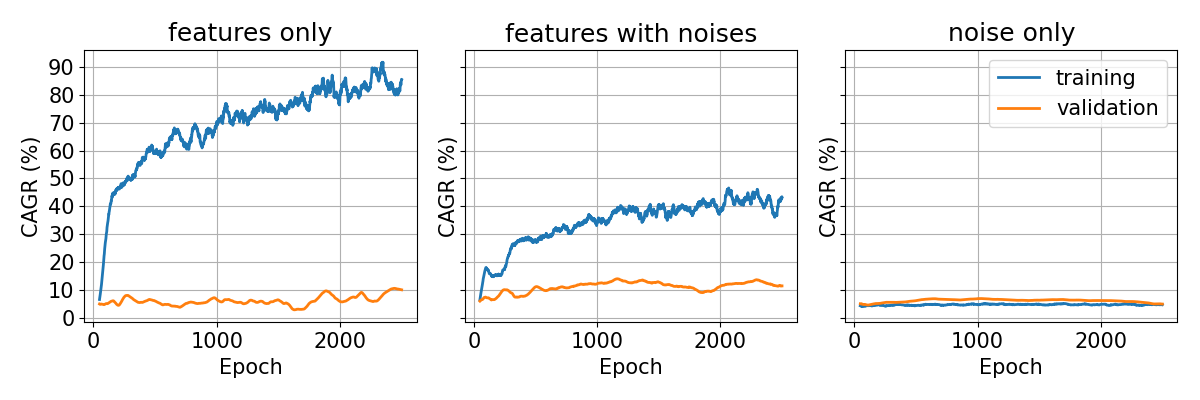
\includegraphics[width=15cm]{images/compare_noise.png}
  \caption{Comparison of using features only, , features with noise, and noise only as states in terms of training and validation CAGR (moving average 50 epochs)}
  \label{fig:noise_diagram}
\end{figure}

\subsection {Portfolio Builder}
The Portfolio Builder Build the portfolio from investments and actions
\subsection {Trading System}
The Trading System measures performances of the given portfolios
\subsection {Reward Provider}
The Reward Provider provides rewards based on the performances of the portfolio and investor preference.